% !TeX program = xelatex
\documentclass[a4paper,10pt]{article}

% ============================================================================
% កញ្ចប់បណ្ណាល័យ (Packages) – តាមលំនាំ NGS Preah Krasang Scenario (2–4 A4 pp.)
% ============================================================================
\usepackage[a4paper, left=0.95cm, right=0.95cm, top=0.80cm, bottom=0.90cm, footskip=0.45cm]{geometry}
\usepackage{amsmath, amssymb}
\usepackage{unicode-math}
\usepackage{fontspec}
\usepackage{array, longtable, multirow, colortbl}
\usepackage[table]{xcolor}
\usepackage{enumitem}
\usepackage{pifont}
\usepackage{fancyhdr}
\usepackage{tikz}
\usetikzlibrary{calc, arrows.meta, positioning, decorations.markings, babel}

% LaTeX 2025 + longtable v4.24 compatibility guard
\makeatletter
\let\@expl@@@mark@update@singlecol@structures@@\relax
\makeatother

% ============================================================================
% ការកំណត់ពុម្ពអក្សរ (Cross-Platform Windows + Cloud fonts/)
% ============================================================================
\providecommand{\NGSFindFonts}{%
  \IfFileExists{C:/Windows/Fonts/cambria.ttc}{%
    \def\NGSSysPath{C:/Windows/Fonts/}%
    \def\NGSUserPath{C:/Users/KIT/AppData/Local/Microsoft/Windows/Fonts/}%
  }{%
    \IfFileExists{./fonts/KhmerOSsiemreap.ttf}{\def\NGSSysPath{./fonts/}\def\NGSUserPath{./fonts/}}{%
    \IfFileExists{../fonts/KhmerOSsiemreap.ttf}{\def\NGSSysPath{../fonts/}\def\NGSUserPath{../fonts/}}{%
    \IfFileExists{../../fonts/KhmerOSsiemreap.ttf}{\def\NGSSysPath{../../fonts/}\def\NGSUserPath{../../fonts/}}{%
    \IfFileExists{../../../fonts/KhmerOSsiemreap.ttf}{\def\NGSSysPath{../../../fonts/}\def\NGSUserPath{../../../fonts/}}{%
    \IfFileExists{../../../../fonts/KhmerOSsiemreap.ttf}{\def\NGSSysPath{../../../../fonts/}\def\NGSUserPath{../../../../fonts/}}{%
    \IfFileExists{../../../../../fonts/KhmerOSsiemreap.ttf}{\def\NGSSysPath{../../../../../fonts/}\def\NGSUserPath{../../../../../fonts/}}{%
    \IfFileExists{../../../../../../fonts/KhmerOSsiemreap.ttf}{\def\NGSSysPath{../../../../../../fonts/}\def\NGSUserPath{../../../../../../fonts/}}{%
      \def\NGSSysPath{../../../../../../../fonts/}\def\NGSUserPath{../../../../../../../fonts/}%
    }}}}}}}%
  }%
}
\NGSFindFonts

\setmathfont[
  Path={\NGSSysPath},
  FontIndex=1,
  Scale=1.02
]{cambria.ttc}

\defaultfontfeatures{Ligatures=TeX}

\setmainfont[
  Path={\NGSUserPath},
  Extension=.ttf,
  Script=Khmer,
  BoldFont={KhmerOSsiemreap},
  BoldFeatures={FakeBold=1.8},
  ItalicFont={KhmerOSsiemreap},
  ItalicFeatures={FakeSlant=0.25},
  BoldItalicFont={KhmerOSsiemreap},
  BoldItalicFeatures={FakeBold=1.8, FakeSlant=0.25}
]{KhmerOSsiemreap}

\newfontfamily\muol[
  Path={\NGSUserPath},
  Extension=.ttf,
  Script=Khmer
]{KhmerOSmuollight}

\newfontfamily\TimesEn[
  Path={\NGSSysPath},
  Extension=.ttf,
  Scale=1.00,
  BoldFont={timesbd},
  ItalicFont={timesi},
  BoldItalicFont={timesbi}
]{times}

\newfontfamily\NagaBold[
  Path={\NGSUserPath},
  Extension=.ttf
]{AKbalthom Naga Bold}

\newfontfamily\CalibriFont[
  Path={\NGSSysPath},
  Extension=.ttf
]{calibri}

\newfontfamily\CourierBullet[
  Path={\NGSSysPath},
  Extension=.ttf
]{cour}
\newcommand{\wcirc}{{\CourierBullet\fontsize{9pt}{10.5pt}\selectfont o}}

\XeTeXlinebreaklocale "km"
\XeTeXlinebreakskip = 0pt plus 1pt minus 0.1pt

% ============================================================================
% ការកំណត់ពណ៌ និងទម្រង់ទំព័រ (Colors & Page Style)
% ============================================================================
\definecolor{stepgray}{HTML}{D9D9D9}
\definecolor{headgray}{HTML}{F2F2F2}
\definecolor{panelgray}{gray}{0.93}
\definecolor{boxgray}{HTML}{D9D9D9}
\definecolor{darkred}{HTML}{C00000}
\definecolor{red5e}{HTML}{FF0000}

\pagestyle{fancy}
\fancyhf{}
\renewcommand{\headrulewidth}{0pt}
\fancyfoot[R]{\CalibriFont\fontsize{10.5pt}{12pt}\selectfont\thepage}

\setlength{\parindent}{0pt}
\setlength{\parskip}{0pt}
\setlength{\tabcolsep}{3.2pt}
\renewcommand{\arraystretch}{1.12}

\newcolumntype{L}[1]{>{\raggedright\arraybackslash}p{#1}}
\newcolumntype{C}[1]{>{\centering\arraybackslash}p{#1}}

% ============================================================================
% ម៉ាក្រូជំនួយ (Helper Macros — គ្មាន \tiny, គ្មាន \\[-2pt])
% ============================================================================
\newcommand{\en}[1]{{\TimesEn #1}}
\newcommand{\enbf}[1]{{\TimesEn\textbf{#1}}}
\newcommand{\unit}[1]{\,\text{\en{#1}}}
\newcommand{\fiveE}[1]{{\NagaBold\fontsize{9.0pt}{12pt}\selectfont\textcolor{red5e}{#1}}}
\newcommand{\timenote}[1]{\textcolor{darkred}{\textit{#1}}}
\newcommand{\cnum}[1]{\mbox{\fontsize{10pt}{11.5pt}\selectfont\ding{\numexpr181+#1\relax}}\hspace{0.15em}}
\newcommand{\ditem}{\tikz[baseline=-0.5ex]\fill (0,0.40ex) -- (0.40ex,0) -- (0,-0.40ex) -- (-0.40ex,0) -- cycle;\hspace{0.25em}}

% ============================================================================
% ម៉ាក្រូគូសរូប TikZ B&W (100% Black Text, font=\footnotesize >= 8.5pt, scale=1.0)
% ============================================================================

% ១. ប្លង់ក្ដារខៀន ៣ តំបន់ (ទទឹង 18.80 cm — ពេញតារាងស្អាត)
\newcommand{\figBoardPlanRN}{%
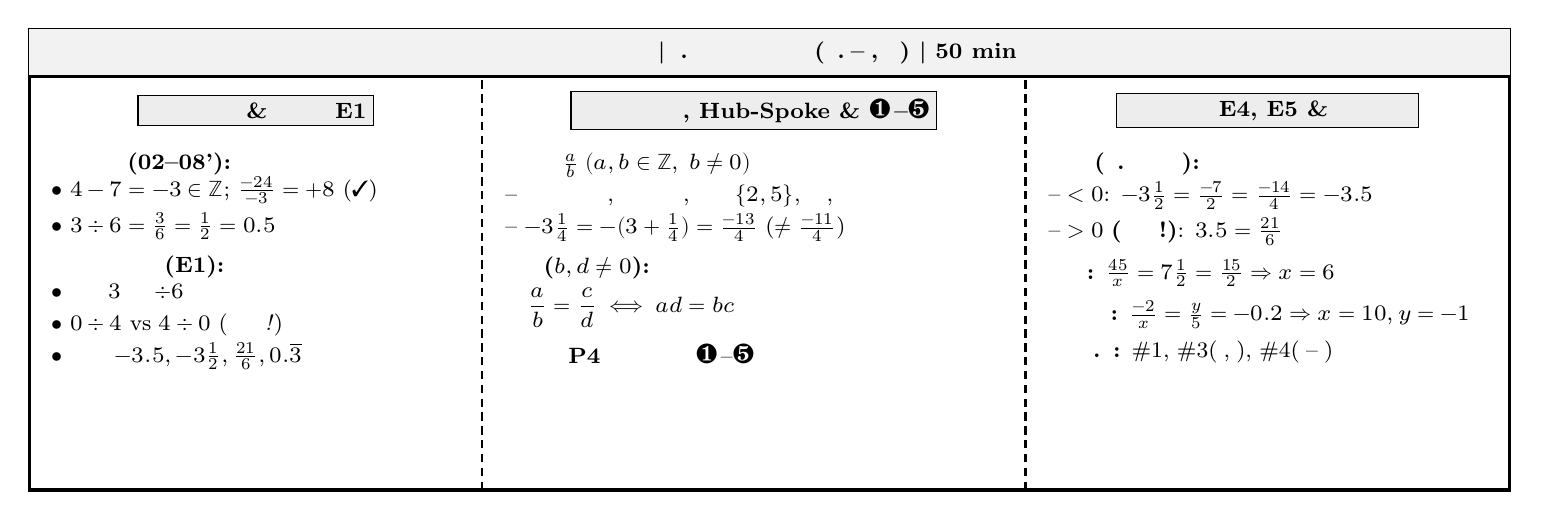
\begin{tikzpicture}[x=1cm, y=1cm, every node/.style={font=\footnotesize, text=black}]
  % Outer Blackboard Frame (spacious 5.85 cm height)
  \draw[black, line width=1.2pt] (0,0) rectangle (18.80, 5.85);
  \fill[headgray] (0, 5.25) rectangle (18.80, 5.85);
  \draw[black, line width=0.85pt] (0, 5.25) -- (18.80, 5.25);
  \node at (9.40, 5.55) {\textbf{មេរៀនទី១ ចំនួនសនិទាន \en{|} ១. សញ្ញាណចំនួនសនិទាន (ទំ.១--២, ១១) \en{|} \en{50 min}}};

  % Vertical dividers for 3 zones
  \draw[black, densely dashed, line width=0.85pt] (5.75, 0) -- (5.75, 5.25);
  \draw[black, densely dashed, line width=0.85pt] (12.65, 0) -- (12.65, 5.25);

  % Zone 1 (Left: Review & E1)
  \node[fill=panelgray, draw=black, line width=0.5pt, inner sep=2.5pt] at (2.875, 4.82) {\textbf{តំបន់ ១៖ រំលឹក \& បេសកកម្ម \en{E1}}};
  \node[anchor=north west, align=left, text width=5.40cm] at (0.16, 4.40) {%
    \textbf{មូលដ្ឋានទី៧ (\en{02--08'}):}\\
    $\bullet\ 4-7 = -3 \in \mathbb{Z}$; $\frac{-24}{-3} = +8$ (\ding{51})\\[2pt]
    $\bullet\ 3\div 6 = \frac{3}{6} = \frac{1}{2} = 0.5$\\[5pt]
    \textbf{ទីផ្សារកំពង់ស្វាយ (\en{E1}):}\\
    $\bullet$ ស្រូវ $3$ បាវ $\div 6$ គ្រួសារ\\[2pt]
    $\bullet$ $0\div 4$ vs $4\div 0$ (\textit{ហាមចែក!})\\[2pt]
    $\bullet$ បំណុល៖ $-3.5,-3\frac{1}{2},\frac{21}{6},0.\overline{3}$};

  % Zone 2 (Center: E2-E3 Definition, Rule, ①–⑤)
  \node[fill=panelgray, draw=black, line width=0.5pt, inner sep=2.5pt] at (9.20, 4.82) {\textbf{តំបន់ ២៖ និយមន័យ, \en{Hub-Spoke} \& \cnum{1}--\cnum{5}}};
  \node[anchor=north west, align=left, text width=6.55cm] at (5.92, 4.40) {%
    \textbf{និយមន័យ៖} $\frac{a}{b}\;(a,b\in\mathbb{Z},\; b\neq 0)$\\[2pt]
    -- ទម្រង់ ៥៖ គត់, រ៉ឺឡាទីបដក, ទសភាគ $\{2,5\}$, ខួប, ចំរុះ\\[2pt]
    -- $-3\frac{1}{4} = -(3+\frac{1}{4}) = \frac{-13}{4}$ ($\neq \frac{-11}{4}$)\\[5pt]
    \textbf{វិធាន ($b,d\neq 0$):}\\[2pt]
    \quad $\dfrac{a}{b}=\dfrac{c}{d} \iff ad=bc$\\[5pt]
    \textbf{បិទផ្ទាំង \en{P4}៖} ធនាគារហេតុផល \cnum{1}--\cnum{5}};

  % Zone 3 (Right: E4-E5 Solutions & HW)
  \node[fill=panelgray, draw=black, line width=0.5pt, inner sep=2.5pt] at (15.725, 4.82) {\textbf{តំបន់ ៣៖ គំរូ \en{E4}, \en{E5} \& កិច្ចការផ្ទះ}};
  \node[anchor=north west, align=left, text width=5.80cm] at (12.82, 4.40) {%
    \textbf{គំរូ ១ (ទំ.២ កែបំពេញ):}\\[2pt]
    -- $<0$: $-3\frac{1}{2}=\frac{-7}{2}=\frac{-14}{4}=-3.5$\\[2pt]
    -- $>0$ \textbf{(កែខ្វះ!)}: $3.5 = \frac{21}{6}$\\[4pt]
    \textbf{គំរូ ២:} $\frac{45}{x}=7\frac{1}{2}=\frac{15}{2} \Rightarrow x=6$\\[4pt]
    \textbf{ប្រតិបត្តិ:} $\frac{-2}{x}=\frac{y}{5}=-0.2 \Rightarrow x=10, y=-1$\\[4pt]
    \textbf{ផ្ទះ ទំ.១១:} \en{\#1, \#3}(ក,គ), \en{\#4}(ក\en{--}ង)};
\end{tikzpicture}}

% ២. រូបផ្ទៀងផ្ទាត់រហ័ស (P1 1:1 Number Line & Cross-Mult Sign Map — width 8.40 cm)
\newcommand{\figScenarioRefRN}{%
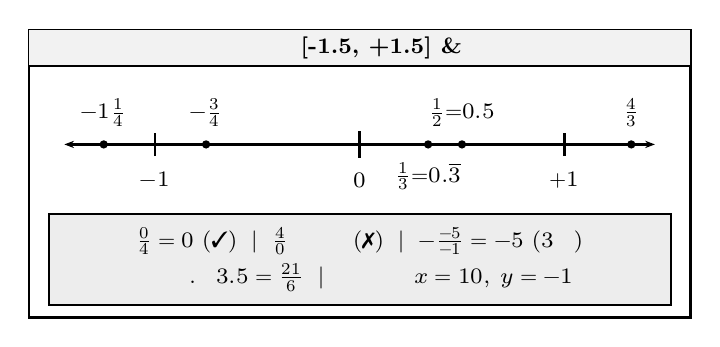
\begin{tikzpicture}[x=1cm, y=1cm, every node/.style={font=\footnotesize, text=black}]
  \draw[black, line width=0.9pt] (0,0) rectangle (8.40, 3.65);
  \fill[headgray] (0, 3.20) rectangle (8.40, 3.65);
  \draw[black, line width=0.8pt] (0, 3.20) -- (8.40, 3.20);
  \node at (4.20, 3.425) {\textbf{ផែនទីបន្ទាត់ភ្លោះ \en{[-1.5, +1.5]} \& តេស្តសញ្ញា}};

  % Number line inside
  \draw[{Stealth[length=3.5pt]}-{Stealth[length=3.5pt]}, black, line width=1.0pt] (0.45, 2.20) -- (7.95, 2.20);
  \draw[black, line width=1.0pt] (1.60, 2.05) -- (1.60, 2.35);
  \node[below=2pt] at (1.60, 2.05) {$-1$};
  \draw[black, line width=1.1pt] (4.20, 2.03) -- (4.20, 2.37);
  \node[below=2pt] at (4.20, 2.03) {$0$};
  \draw[black, line width=1.0pt] (6.80, 2.05) -- (6.80, 2.35);
  \node[below=2pt] at (6.80, 2.05) {$+1$};
  % Points
  \fill[black] (0.95, 2.20) circle (1.5pt);
  \node[above=3pt] at (0.95, 2.20) {$-1\frac{1}{4}$};
  \fill[black] (2.25, 2.20) circle (1.5pt);
  \node[above=3pt] at (2.25, 2.20) {$-\frac{3}{4}$};
  \fill[black] (5.07, 2.20) circle (1.5pt);
  \node[below=3pt] at (5.07, 2.20) {$\frac{1}{3}{=}0.\overline{3}$};
  \fill[black] (5.50, 2.20) circle (1.5pt);
  \node[above=3pt] at (5.50, 2.20) {$\frac{1}{2}{=}0.5$};
  \fill[black] (7.65, 2.20) circle (1.5pt);
  \node[above=3pt] at (7.65, 2.20) {$\frac{4}{3}$};

  % Bottom Quick Reference strip (taller vertical box clearance)
  \draw[black, line width=0.75pt, fill=panelgray] (0.25, 0.16) rectangle (8.15, 1.32);
  \node[align=center] at (4.20, 0.74) {$\frac{0}{4}=0$ (\ding{51}) \;\textbar{}\; $\frac{4}{0}$ គ្មានន័យ (\ding{55}) \;\textbar{}\; $-\frac{-5}{-1} = -5$ ($3$ ដក)\\[2pt]
  បំពេញទំ.២៖ $3.5 = \frac{21}{6}$ \;\textbar{}\; ប្រតិបត្តិ៖ $x=10,\; y=-1$};
\end{tikzpicture}}

\begin{document}
\fontsize{9.5pt}{13.6pt}\selectfont

% ============================================================================
% ក្បាលទំព័រ (Header & Metadata)
% ============================================================================
\begin{center}
{\muol\fontsize{11pt}{15pt}\selectfont សេណារីយ៉ូនៃការបង្រៀន \enbf{(Teaching Scenario -- RN1)}}
\end{center}
\vspace{3pt}

% ទទឹងតារាង 1.95 + 6.75 + 1.85 + 7.45 = 18.00 cm + 8*3.2pt = 18.90 cm (គ្មាន overfull)
\noindent\begin{tabular}{|L{1.95cm}|L{6.75cm}|L{1.85cm}|L{7.45cm}|}
\hline
\rowcolor{headgray}
\textbf{សាលារៀន៖} & អនុវិទ្យាល័យព្រះក្រសាំង (កំពង់ស្វាយ--កំពង់ធំ) & \textbf{មុខវិជ្ជា៖} & គណិតវិទ្យា ថ្នាក់ទី៨ (ផ្នែកពីជគណិត) \\
\hline
\textbf{មេរៀន៖} & \textbf{មេរៀនទី១ ចំនួនសនិទាន (១. សញ្ញាណចំនួនសនិទាន)} & \textbf{រយៈពេល៖} & \textcolor{darkred}{\textbf{១ ម៉ោងសិក្សា (៥០ នាទី)}} \textbullet\ ទំ.១--២, ១១ \\
\hline
\textbf{គ្រូបង្រៀន៖} & ហុក ប៊ុនថែន & \textbf{កាលបរិច្ឆេទ៖} & ថ្ងៃចន្ទ ទី២ ខែវិច្ឆិកា ឆ្នាំ២០២៦ (៨រោច ខែអស្សុជ ២៥៧០) \\
\hline
\end{tabular}

\vspace{5pt}
{\muol ផ្នែកទី ១៖ លំដាប់ឈុតឆាកបង្រៀន ៥០ នាទី \enbf{(}៨ ឈុតលម្អិត\enbf{)}}
\vspace{2pt}

% ============================================================================
% ផ្នែកទី ១៖ តារាងឈុតឆាក (8 Chronological Scenes = 50 min, 17.80 + 10*3.2pt = 18.93 cm)
% ============================================================================
\begin{longtable}{|C{1.25cm}|L{2.65cm}|C{0.90cm}|L{8.35cm}|L{4.65cm}|}
\hline
\rowcolor{stepgray}
\textbf{ម៉ោង} & \textbf{ឈុត / ជំហាន \enbf{5E}} & \textbf{នាទី} & \textbf{សកម្មភាពបង្រៀន និងសំណួរ--ចម្លើយគំរូ (គ្រូ--សិស្ស)} & \textbf{សម្ភារៈ និងកំណត់ចំណាំ / \enbf{Warrant}} \\
\hline
\endfirsthead
\hline
\rowcolor{stepgray}
\textbf{ម៉ោង} & \textbf{ឈុត / ជំហាន \enbf{5E}} & \textbf{នាទី} & \textbf{សកម្មភាពបង្រៀន និងសំណួរ--ចម្លើយគំរូ (គ្រូ--សិស្ស)} & \textbf{សម្ភារៈ និងកំណត់ចំណាំ / \enbf{Warrant}} \\
\hline
\endhead
\hline
\endfoot
\hline
\endlastfoot

% --- ឈុតទី ១ ---
00--02 &
\textbf{ឈុតទី ១}\par
ជំហានទី១៖\par
រដ្ឋបាលថ្នាក់ &
២ &
\ditem គ្រូពិនិត្យអវត្តមាន អនាម័យថ្នាក់ និងចាត់ក្រុម ៣ នាក់ជា \textbf{«ក្រុមវិស្វករសហគមន៍»}។\par\vspace{2pt}
\ditem \textbf{គ្រូ៖} «ប្អូនដាក់បន្ទាត់ \en{cm} និងកន្ត្រៃឱ្យមានរបៀប រួចផ្កាប់ក្រដាស \en{P1 (1:1)} មុនគ្រូប្រាប់!»\par\vspace{2pt}
\ditem \textbf{សិស្ស៖} ប្រធានថ្នាក់រាយការណ៍អវត្តមាន និងក្រុមត្រៀមឧបករណ៍។ &
\wcirc\ រក្សាសុវត្ថិភាពកន្ត្រៃ/បន្ទាត់។\par\vspace{2pt}
\wcirc\ ចែកសន្លឹក \en{P1 (1:1)} ផ្កាប់មុខកុំឱ្យរំខានចក្ខុមុន \fiveE{E2}។ \\[3pt]
\hline

% --- ឈុតទី ២ក & ២ខ ---
02--05 &
\textbf{ឈុតទី ២ក}\par
ជំហានទី២៖\par
ពិនិត្យមូលដ្ឋាន\par
ថ្នាក់ទី៧ &
$\le$៣ &
\ditem \textbf{ក. មូលដ្ឋានទី៧ ($\le 3'$):} គ្រូសរសេរ $4-7$, $\frac{-24}{-3}$, និង $3\div 6$។\par
\textbf{គ្រូ៖} «តើ $\frac{-24}{-3}$ ស្មើ $8$ ឬ $-8$? ហេតុអ្វី?»\par
\textbf{សិស្ស៖} «$4-7=-3\in\mathbb{Z}$; $\frac{-24}{-3}=+8$ ព្រោះដកចែកដកបានបូក; $3\div 6=\frac{3}{6}=\frac{1}{2}$!» &
\wcirc\ កំណែ/ផ្ទៀង $\le 3'$ កុំឱ្យអូសបន្លាយ។\par\vspace{2pt}
\wcirc\ កាត់បន្ថយអន្ទាក់សញ្ញា \cnum{2} ($\frac{-24}{-3}=+8$, \en{Yetim \& Alkan, 2013})។ \\[3pt]

05--08 &
\textbf{ឈុតទី ២ខ}\par
ជំហានទី២៖\par
រំលឹកមេរៀនទាក់ទង &
៣ &
\ditem \textbf{ខ. រំលឹក ($3'$):} ទម្រង់ប្រភាគនៃចំនួនគត់ និងទសភាគដប់។\par
\textbf{គ្រូ៖} «តើ $0.5$ សរសេរជាប្រភាគភាគបែង $10$ ដូចម្ដេច? ចុះ $-\frac{5}{1}$?»\par
\textbf{សិស្ស៖} «$0.5=\frac{5}{10}=\frac{1}{2}$; $5=\frac{5}{1}$ និង $-5=\frac{-5}{1}=\frac{5}{-1}=-\frac{5}{1}$!» &
\wcirc\ រំលឹកទម្រង់ $n=\frac{n}{1}$ មុនចូល $\mathbb{Q}$ (\en{Rizos \& Adam, 2022})។ \\[3pt]
\hline

% --- ឈុតទី ៣ ---
08--11 &
\textbf{ឈុតទី ៣}\par
\fiveE{E1 Engage}\par
ទីផ្សារសហគមន៍\par
កំពង់ស្វាយ &
៣ &
\ditem គ្រូលើកបេសកកម្ម \textbf{«ទីផ្សារសហគមន៍កំពង់ស្វាយ»}៖ ស្រូវ $3$ បាវ $\div 6$ គ្រួសារ ($3\div 6$), ផ្លែឈើ $4\unit{kg} \div 0$ នាក់ ($4\div 0$), បញ្ជីបំណុល $-3.5, -3\frac{1}{2}, \frac{21}{6}, 0.\overline{3}$។\par\vspace{2pt}
\ditem \textbf{សំណួរ ១៖} «តើ $\frac{3}{6}, -3, 0.5, 0.\overline{3}$ ជារបស់ក្រុមតែមួយឬទេ?»\par
\ditem \textbf{សំណួរ ២ (\en{POE}):} «ហេតុអ្វី $0\div 4$ ចែកបាន តែ $4\div 0$ ហាមចែក?»\par
\ditem \textbf{សិស្ស៖} ទស្សន៍ទាយខុសៗគ្នា គ្រូកត់ទុក \textbf{មិនទាន់ប្រាប់ចម្លើយ}។ &
\wcirc\ បង្កើតជម្លោះគំនិតជាក់ស្ដែងក្នុងសហគមន៍។\par\vspace{2pt}
\wcirc\ កត់ទុកការទស្សន៍ទាយ ដើម្បីត្រឡប់បិទនៅ \fiveE{E5}។ \\[3pt]
\hline

% --- ឈុតទី ៤ (ក) ---
11--17 &
\textbf{ឈុតទី ៤ក}\par
\fiveE{E2 Explore}\par
ស.១ បត់បន្ទះ \en{1:1} &
៦ &
\ditem \textbf{បត់ \en{1:1} (\en{P1}):} ក្រុមផ្ទៀងក្រិត \en{5.00 cm (Actual Size 100\%)} រួចកាត់បន្ទះ $1$ ឯកតា ($=6.00\unit{cm}$) បត់ជា $2, 3, 4$ ផ្នែកស្មើ។\par\vspace{2pt}
\ditem ដាក់លើបន្ទាត់ភ្លោះ $[-1.5, +1.5]$៖ $\frac{1}{2}=0.5=\frac{5}{10}=\frac{3}{6}$, $\frac{1}{3}=0.\overline{3}$, $\frac{4}{3}=1\frac{1}{3}=1.\overline{3}$, និងឆ្លុះខាងឆ្វេង $0$ ($-$) រក $-\frac{3}{4}=-0.75$ និង $-1\frac{1}{4}=-\frac{5}{4}$។\par\vspace{2pt}
\ditem \textbf{សិស្ស៖} ឃើញច្បាស់ថា $\frac{1}{2}, 0.5, \frac{5}{10}$ ចង្អុលត្រង់ទីតាំងតែមួយ! &
\wcirc\ សន្លឹក \en{P1 1:1} ($1\text{ unit}=6.00\unit{cm}$), កន្ត្រៃ, បន្ទាត់ (\en{Pearn, 2007; Gorman et al., 2025})។ \\[3pt]

% --- ឈុតទី ៤ (ខ) ---
17--22 &
\textbf{ឈុតទី ៤ខ}\par
\fiveE{E2 Explore}\par
ស.២ \en{Dual POE} &
៥ &
\ditem \textbf{\en{POE 2A} (អន្ទាក់សូន្យ):} ទាយ $\frac{0}{4}, \frac{4}{0}, \frac{0}{0}$ រួចផ្ទៀងតាមច្រាសផលគុណ $k\times b = a$៖\par
-- $\frac{0}{4}=k \iff k\times 4=0 \Rightarrow k=0$ (\ding{51});\par
-- $\frac{4}{0}=k \iff k\times 0=4$ (គ្មាន $k \Rightarrow$ គ្មានន័យ! $b\neq 0$); $\frac{0}{0}$ មិនកំណត់។\par\vspace{2pt}
\ditem \textbf{\en{POE 2B} (ទសភាគខួប \& សញ្ញាចម្រុះ):}\par
-- កែការភាន់ច្រឡំទំ.១៖ $\frac{1}{2}=0.5$ ក៏បឋមនឹងគ្នា តែដាច់ព្រោះភាគបែងជា $2$ (\textit{លុះត្រាតែក្រៅពី $\{2,5\}$ ទើបខួប!});\par
-- $-3\frac{1}{4} = -(3+\frac{1}{4}) = \frac{-13}{4}$ (ហាម $\frac{-3\times 4+1}{4}=\frac{-11}{4}$!)។ &
\wcirc\ \en{Karakuş \& Aydın (2019)}៖ ច្រាសផលគុណ។\par\vspace{2pt}
\wcirc\ \en{Susiswo et al. (2021)}៖ ឧបសគ្គសញ្ញាចម្រុះដក។ \\[3pt]
\hline

% --- ឈុតទី ៥ក & ៥ខ ---
22--25 &
\textbf{ឈុតទី ៥ក}\par
\fiveE{E3 Explain}\par
និយមន័យ \& \en{5} ទម្រង់ &
៣ &
\ditem គ្រូដឹកនាំបង្គុំនិយមន័យ (ទំ.១)៖ «ចំនួនសនិទានជាចំនួនមានទម្រង់ $\frac{a}{b}$ ដែល $a,b\in\mathbb{Z}$ និង $b\neq 0$» ភ្ជាប់ដ្យាក្រាម \textbf{\en{Hub-and-Spoke}} ទាំង ៥ ទម្រង់ (គត់, រ៉ឺឡាទីបដក, ទសភាគ $\{2,5\}$, ខួប, ចំរុះ)។ &
\wcirc\ បិទផ្ទាំង \textbf{\en{P4} (Anchor Poster)} (\en{Xu et al., 2026})។ \\[3pt]

25--28 &
\textbf{ឈុតទី ៥ខ}\par
\fiveE{E3 Explain}\par
វិធាន $ad=bc$ \& \cnum{1}--\cnum{5} &
៣ &
\ditem បង្ហាញវិធានសមភាព (ទំ.២ កែលក្ខខណ្ឌ $b,d\neq 0$)៖ $\frac{a}{b}=\frac{c}{d} \iff ad=bc$។\par\vspace{2pt}
\ditem \textbf{សិស្ស៖} សង្ខេបនិយមន័យ និងរំលឹក \textbf{ធនាគារហេតុផល \cnum{1}--\cnum{5}}។ &
\wcirc\ ភ្ជាប់ធនាគារហេតុផល \cnum{1}--\cnum{5} មុនចូល \fiveE{E4}។ \\[3pt]
\hline

% --- ឈុតទី ៦ ---
28--34 &
\textbf{ឈុតទី ៦ក}\par
\fiveE{E4 Elaborate}\par
គំរូទី ១ (ទំ.២ កែ)\par
+ \en{[tracing]} &
៦ &
\ditem ចែកកាត \textbf{\en{P2 (2-up)} «៣ ជំហានស៊ើបអង្កេត»}៖\par
\ditem \textbf{គំរូទី ១ (កែបំពេញទំ.២):} ផ្គុំ $-3\frac{1}{2}, 3.5, \frac{-7}{2}, \frac{-14}{4}, -3.5, \frac{21}{6}$ ដោយ \en{[tracing]}៖\par
-- ក្រុម $<0$៖ $-3\frac{1}{2}=\frac{-7}{2}=\frac{-14}{4}=-3.5$ \mbox{(\cnum{3}, \cnum{5});}\par
-- ក្រុម $>0$ (\textbf{បំពេញសៀវភៅខ្វះ!})៖ $3.5=\frac{35}{10}=\frac{7}{2}=\frac{21}{6}$! &
\wcirc\ \en{P2 (2-up)} កាត ៣ ជំហាន + \en{[tracing]} (\en{Barbieri et al., 2023; Yeo \& Tzeng, 2019})។ \\[3pt]

34--38 &
\textbf{ឈុតទី ៦ខ}\par
\fiveE{E4 Elaborate}\par
គំរូទី ២ \& \en{EIA} &
៤ &
\ditem \textbf{គំរូទី ២:} $\frac{45}{x}=7\frac{1}{2}=\frac{15}{2} \Rightarrow 15x=90 \Rightarrow x=6\neq 0$ \mbox{(\cnum{1}, \cnum{4})។}\par
\ditem \textbf{\en{EIA} 30s:} ហេតុអ្វី $-3\frac{1}{2}=-\frac{7}{2}\neq -\frac{5}{2}$ និងត្រូវផ្គុំ $3.5=\frac{21}{6}$ ផង? &
\wcirc\ ពង្រឹងការពន្យល់ខ្លួនឯងតាម \cnum{1}, \cnum{3}, \cnum{4}, \cnum{5}។ \\[3pt]
\hline

% --- ឈុតទី ៧ (ក) ---
38--43 &
\textbf{ឈុតទី ៧ក}\par
\fiveE{E5 Evaluate}\par
\en{Relay 3} តួនាទី\par
(ប្រតិបត្តិ ទំ.២) &
៥ &
\ditem ចែកសន្លឹក \textbf{\en{P3 (2-up)}} ធ្វើ \textbf{ប្រតិបត្តិ (ទំ.២)} រក $x, y$ ដើម្បីឱ្យ $\frac{-2}{x}, \frac{y}{5}, -0.2$ ស្មើគ្នា៖\par
-- \textbf{តួនាទី ១ (\en{Pause-Ask}):} \en{[tracing]} $-0.2=\frac{-2}{10}=\frac{-1}{5}$ និងពិនិត្យ $x\neq 0$;\par
-- \textbf{តួនាទី ២:} គណនា $\frac{-2}{x}=\frac{-1}{5}\Rightarrow x=10$ និង $\frac{y}{5}=\frac{-1}{5}\Rightarrow y=-1$ (\cnum{4});\par
-- \textbf{តួនាទី ៣ (\en{Pause-Review}):} រាប់សញ្ញាដក $-\frac{-5}{-1}=-5$ (\cnum{2}) និង \textbf{បិទ \fiveE{E1}} ($3\div 6, -3, 0.5, 0.\overline{3}\in\mathbb{Q}$ តែ $4\div 0$ ហាម!)។ &
\wcirc\ \en{P3 (2-up)} Relay ៣ តួនាទី។\par\vspace{2pt}
\wcirc\ ពិនិត្យវិន័យ \en{Pause-Ask / Pause-Review}។ \\[3pt]

% --- ឈុតទី ៧ (ខ) ---
43--48 &
\textbf{ឈុតទី ៧ខ}\par
\fiveE{E5 Evaluate}\par
កាត \en{A--D} \&\par
សំបុត្រចេញ &
៥ &
\ditem \textbf{កាត \en{A--D} (\en{P5}):} លើកកាត \mbox{A (\ding{51} $-3\frac{1}{4}=\frac{-13}{4}=-3.25$),} \mbox{B (\ding{55} $\frac{4}{0}=0$),} \mbox{C (\ding{55} $-7, 0.\overline{3}\notin\mathbb{Q}$),} \mbox{D (\ding{55} $0.25<0 / -3\frac{1}{4}=\frac{-11}{4}$)។}\par\vspace{2pt}
\ditem \textbf{សំបុត្រចេញ (60--90s):} ១) $-2\frac{3}{4}=\frac{-11}{4}=-2.75$; ២) $\frac{0}{-5}=0\in\mathbb{Q}$ vs $\frac{-5}{0}$ គ្មានន័យ; ៣) $\frac{12}{m}=-0.6\Rightarrow m=-20$។ &
\wcirc\ \en{McLaren et al. (2012)}: កំហុស \en{\textit{Negz/Megz}}។\par\vspace{2pt}
\wcirc\ ប្រមូលសំបុត្រចេញជាភស្តុតាងវាយតម្លៃ។ \\[3pt]
\hline

% --- ឈុតទី ៨ ---
48--50 &
\textbf{ឈុតទី ៨}\par
ជំហានទី៥៖\par
កិច្ចការផ្ទះ &
២ &
\ditem ចែកប័ណ្ណ \textbf{\en{P6 (4-up)} (ទំ.១១)}៖ \textbf{\#1} រកចំនួនស្មើ $-5$ ($\frac{-5}{1},\frac{5}{1},\frac{5}{-1},-\frac{5}{1},\frac{-5}{-1},-\frac{-5}{1},-\frac{-5}{-1}$ — រាប់សញ្ញាដកគត់/សេស!), \textbf{\#3(ក,គ)} ($28.45,\; 1\frac{19}{50}$), \textbf{\#4(ក--ង)} ($\frac{7}{100},\frac{13}{10,000},\frac{3}{2^4},\frac{7}{2^3\cdot 5},\frac{17}{652}$ — កត្តា $652=2^2\times 163$)។\par\vspace{2pt}
\ditem \textbf{បណ្ដាំផ្ញើ៖} «អានជាមុន \textbf{២.១ ការប្រៀបធៀបចំនួនសនិទាន (ទំ.២--៣)}!» &
\wcirc\ ចំណាយពេល $\le 2$ នាទី។\par\vspace{2pt}
\wcirc\ រំលឹក $\#3(\text{ខ,ឃ,ង})$ ជាខួបសម្រាប់ម៉ោងបន្ទាប់។ \\[3pt]
\hline
\end{longtable}

\vspace{4pt}
{\muol ផ្នែកទី ២៖ ប្លង់ក្ដារខៀនស្តង់ដារ ៣ តំបន់ \enbf{(3-Zone Blackboard Plan)}}
\vspace{3pt}

\noindent\centering\figBoardPlanRN\par

\vspace{6pt}
\raggedright
% ============================================================================
% ផ្នែកទី ៣៖ បញ្ជីសម្ភារៈ B&W (ចប់ស្អាតលើទំព័រទី ២ ដើម្បីឱ្យពេញក្រដាស >= 90%)
% ============================================================================
{\muol ផ្នែកទី ៣៖ បញ្ជីសម្ភារៈ \enbf{B\&W} និងឧបករណ៍តុពិសោធន៍}\\[3pt]
{\fontsize{9.2pt}{13.2pt}\selectfont
\ditem \textbf{\en{P1 (1:1 Actual Size 100\%)}៖} ក្រិតផ្ទៀង $5.00\unit{cm}$, បន្ទះកាត់ $1\text{ unit}=6.00\unit{cm}$ (ពេញ, $2/4$, $3$, $10$ ផ្នែក), បន្ទាត់ភ្លោះ $[-1.5, +1.5]$, និងតារាង \en{Dual POE 2A--2B} ។\\[2pt]
\ditem \textbf{\en{P2 \& P3 (2-up)}៖} កាត ៣ ជំហាន \en{E4} (គំរូ ១ កែ $3.5=\frac{21}{6}$ \& គំរូ ២) និងសន្លឹក \en{Relay 3} តួនាទី \en{E5} (ប្រតិបត្តិ $x=10, y=-1$, រាប់ដក $-\frac{-5}{-1}=-5$) ។\\[2pt]
\ditem \textbf{\en{P4, P5, P6}៖} ផ្ទាំង \en{Hub-and-Spoke} \& \cnum{1}--\cnum{5}, កាត \en{A--D} + សំបុត្រចេញ ៣ សំណួរ (\en{2-up}), និងប័ណ្ណកិច្ចការផ្ទះ ទំ.១១ (\en{4-up}) ។\\[2pt]
\ditem \textbf{ឧបករណ៍តុ ៣ នាក់៖} កន្ត្រៃ ១, បន្ទាត់ \en{cm} ១, ខ្មៅដៃ \en{[tracing]} (គ្មានតម្រូវការហ្វឺតពណ៌លើសន្លឹក \en{B\&W}) ។
}

\vspace{7pt}
% ============================================================================
% ផ្នែកទី ៤៖ រូបផ្ទៀងរហ័ស & ការភាន់ច្រឡំសិស្ស (Empirical — ទំព័រទី ៣ ពេញទទឹង)
% ============================================================================
\noindent\begin{minipage}[t]{8.6cm}
{\muol រូបផ្ទៀងរហ័ស \enbf{\&} គោលដៅបិទ \enbf{E1}}\\[4pt]
\figScenarioRefRN
\end{minipage}\hfill
\begin{minipage}[t]{9.9cm}
{\muol តារាងពិនិត្យវិន័យ និងសូចនាករសម្រេច ៥០ នាទី}\\[4pt]
{\fontsize{9.2pt}{13.4pt}\selectfont
\renewcommand{\arraystretch}{1.15}
\begin{tabular}{|L{3.10cm}|L{6.25cm}|}
\hline
\rowcolor{stepgray}
\textbf{ដំណាក់កាល} & \textbf{ចំណុចផ្ទៀងផ្ទាត់ (\en{Pause-Ask / Gate})} \\
\hline
\textbf{E1--E2 ($08$--$22'$)} & ទប់ស្កាត់ $\frac{4}{0}=0$, កែ $\{2,5\}$ vs $3$, បង្ហាញ $-3\frac{1}{4}=\frac{-13}{4}$ ។ \\
\hline
\textbf{E3 ($22$--$28'$)} & បង្គុំ $\frac{a}{b}\;(b\neq 0)$, \en{Hub-and-Spoke} ៥ ទម្រង់, $ad=bc\;(b,d\neq 0)$ ។ \\
\hline
\textbf{E4--E5 ($28$--$48'$)} & \en{[tracing]} កែខ្វះ $3.5=\frac{21}{6}$; $x=6$; $(x,y)=(10,-1)$; កាត \en{A--D} ។ \\
\hline
\textbf{ផ្ទះ ($\le 2'$)} & ចែក \en{P6} ទំ.១១ \en{\#1, \#3}(ក,គ), \en{\#4}(ក\en{--}ង) (កត្តា $652$) ។ \\
\hline
\end{tabular}}
\end{minipage}

\vspace{8pt}
{\muol ផ្នែកទី ៤៖ ការភាន់ច្រឡំសិស្ស និងវិធានការដោះស្រាយ \enbf{(Empirical Misconceptions)}}\\[4pt]
{\fontsize{9.5pt}{13.6pt}\selectfont
\renewcommand{\arraystretch}{1.16}
\begin{tabular}{|L{6.80cm}|L{11.55cm}|}
\hline
\rowcolor{stepgray}
\textbf{ការភាន់ច្រឡំ (\en{Empirical Finding})} & \textbf{វិធានការបង្ការ និងដោះស្រាយជាក់ស្ដែងក្នុងថ្នាក់ \enbf{RN1}} \\
\hline
\textbf{១. មិនចាត់ទុកគត់/ខួប $\in\mathbb{Q}$៖} កាត់ចោល $2, -7, 0.\overline{3}$ និងភ្លេច $n=\frac{n}{1}$ (\en{Yetim \& Alkan, 2013}: 72.6--80.8\%; \en{Rizos \& Adam, 2022}: 30\%)។ & បង្គុំដ្យាក្រាម \en{Hub-and-Spoke} (\en{Xu et al., 2026}), រំលឹក $5=\frac{5}{1}$, បត់បន្ទះ $\frac{1}{3}=0.\overline{3}$ លើ \en{P1} និងដាក់កាត \en{C} នៅ \en{E5}។ \\
\hline
\textbf{២. អន្ទាក់ $\frac{4}{0}=0$ និង $\frac{0}{4}=4$៖} ស្រាយដោយក្បួនចាំស្ងួត (\en{Karakuş \& Aydın, 2019}: 39--51\%; \en{Yetim \& Alkan, 2013}: 31.5\%)។ & ប្រើ \en{POE 2A} សាករក $k\times 0 = 4$ ឱ្យសិស្សឃើញផ្ទាល់ថាគ្មាន $k \Rightarrow b\neq 0$ និងដាក់កាត \en{B} នៅ \en{E5}។ \\
\hline
\textbf{៣. ឧបសគ្គសញ្ញាចម្រុះដក និង \en{\textit{Negz}}៖} គណនា $-3\frac{1}{4}=\frac{-11}{4}$ និង $\frac{-24}{-3}=-8$ (\en{Susiswo et al., 2021; McLaren et al., 2012})។ & បង្រៀន $-m\frac{p}{q}=-(m+\frac{p}{q})$ ក្នុង \en{POE 2B}, ញែកក្រុម $<0$ vs $>0$ ក្នុងគំរូ ១, រាប់ដកគត់/សេសក្នុង \en{P3, P6} និងកាត \en{D}។ \\
\hline
\textbf{៤. បម្លែងទម្រង់តាមក្បួនស្ងួត៖} ខុស $82.2\%$ (\en{Lemonidis \& Pilianidis, 2020}: 68.9\% កំហុសនីតិវិធី; \en{Žakelj \& Klančar, 2024})។ & ផ្ទៀងបន្ទះ \en{1:1} លើបន្ទាត់ភ្លោះ (\en{Siegler et al., 2011}), បង្រៀនលក្ខខណ្ឌកត្តា $\{2,5\}$ (គំរូ \#4ង $652$) និង \en{[tracing]}។ \\
\hline
\end{tabular}}

\vspace{10pt}
\hfill
\begin{minipage}{9.8cm}
  {\centering
    ថ្ងៃចន្ទ ៨រោច ខែអស្សុជ ឆ្នាំមមី អដ្ឋស័ក ពុទ្ធសករាជ ២៥៧០\\[2pt]
    កំពង់ស្វាយ, ថ្ងៃទី២ ខែវិច្ឆិកា ឆ្នាំ២០២៦\\[3pt]
    {\muol គ្រូបង្រៀន}\par}
  \vspace{32pt}
  \hfill{\muol ហុក ប៊ុនថែន}\hspace*{1.4cm}
\end{minipage}

\end{document}
